\documentclass[11pt]{article}
\usepackage[letterpaper,margin=0.85in]{geometry}
\usepackage{amsmath,amssymb,booktabs,longtable,array,graphicx,url,hyperref,etoolbox,needspace}
\BeforeBeginEnvironment{table}{\par}
\AfterEndEnvironment{table}{\par}
\hypersetup{hidelinks}
\title{Supplementary Material\\\large Protocol-Constrained Residual Estimation for Rigid-Body Inference: Strong Baselines and Visual Controls}
\author{Hyojin Park, Nam-Hyun Yoo, and Jinhong Yang}
\date{}
\begin{document}\maketitle
\noindent This supplement provides implementation details, statistical definitions, dataset-selection information, and instructions for reproducing the saved-result calculations associated with the main article.

\section{Claim-to-artifact map}
\begin{longtable}{p{.16\textwidth}p{.37\textwidth}p{.38\textwidth}}
\caption{Evidence supporting the main article and its interpretation.}\\
\toprule Claim & Evidence in the package & Permitted interpretation\\\midrule\endhead
C1: 20.30\% full-model improvement versus profiled MAP & Profiled-MAP losses and follow-up focal statistics; paired family replay & Synthetic new-geometry analytic action utility; most gain is numerical.\\
C2: 1.07\% main visual increment & Matched numerical and complete-model family losses & Small selected-feature increment; the two-sided interval includes zero.\\
C2b: 4.27\% public increment & Public error archive and original bootstrap draws & Task-specific fitting followed by offline episode evaluation; not zero-shot or validated object-level transfer.\\
C3: proper scores and coverage & Main and public result JSON; main cached property means/covariances; selected public radius & Main posterior scores reproduced and mean-fixed sensitivity added; no conformal guarantee.\\
Capacity: 1,936 & Bundled residual checkpoint weight and intercept shapes & Stored residual coefficients only; 1,694 can affect final outputs outside the disabled branch.\\
Real-video boundary & Saved 33-video, 11-family result JSON & Direct domain inversion and nonsignificant bridge; diagnostic only.\\\bottomrule
\end{longtable}
The evidence paths retain their original directory layout under \texttt{evidence/}. The accompanying evidence inventory provides file checksums and the retained temporal audit. SHA-256 identifies bytes, not independently verified creation time.

\section{Training and label-access sequence}
\begin{enumerate}
\item Construct observation-only numeric inputs and frozen observation-decoder features. Known force, timing, camera/setup, prior, and linearization inputs are explicit information, not learned visual evidence.
\item For each outer training family partition, fit feature means/scales and the numerical residual heads to anchor-standardized physical targets. Clip the numerical training prediction to two anchor standard deviations.
\item Fit the visual heads on the remaining \emph{in-sample} numerical training residual. Clip their prediction to one standard deviation and multiply by 0.25.
\item Apply both heads to the outer test families, enforce the protocol mask, disable the complete correction for generalized bounce, and calculate accepted-update covariance inflation.
\item Select the final configuration on development data, fit the stored checkpoint, and retain the later confirmation losses separately.
\end{enumerate}
The public extension uses the analogous numerical-then-visual residual, with an additional gate. Four inner folds generate component predictions for gate targets within each of five outer folds. Five candidate gate penalties are scored using those outer predictions. Earlier component selection and gate-penalty selection reuse the 53-episode development cohort. This does not constitute fully nested model-selection validation.

The public radius uses the selected 53 out-of-fold errors at rank 49. Fitting, selection, and residual calibration share the development cohort. The confirmation cohort does not set the radius. We use the term \emph{development-calibrated empirical radial region}, without claiming split-conformal, CV+, or jackknife+ guarantees.

\section{Feature and solver implementation details}
The main numerical feature dictionary has 24 entries per frame. Nine time-dependent entries are active-axis position, relative position, velocity, velocity difference, log observation noise, time, time increment, time since force switch, and switch indicator. Fifteen repeated setup entries are two forces, one switch time, three active flags, three prior means, three log prior scales, and three prior-normalized linearization coordinates. Flattening eight frames gives 192 inputs. The numerical readout uses no selected visual-residual channel, although it depends on the supplied physical setup and prior specification.

The visual extraction runs the vision component of Qwen3-VL-2B-Instruct, not its text decoder. The model commit is \texttt{89644892e4d85e24eaac8bacfd4f463576704203}; full model weights are not distributed in this package. Separate image processing uses a $512^2$ pixel budget, a $32\times32$ grid, and BF16 vision evaluation. The frozen observation decoder projects encoder features, combines RGB and tracking, transports temporal state, and pools with spatial attention. The 32 pooled values are states before its static/dynamic correction heads. They are not 32 raw language-model channels. Their temporal mean and normalized static/dynamic position corrections form the 48-dimensional main view.

Relevant source excerpts are:
\begin{itemize}
\item \path{stream_com_internal_features_v16.py}
\item \path{com_observation_decoder_v8.py}
\item \path{train_com_physics_internal_readout_v12.py}
\item \path{sequential_robust_readout_v22.py}
\end{itemize}
The frozen observation decoder was learned before the residual stage; its parameters must not be hidden inside the 1,936-coefficient claim.

The main robust control computes standardized innovations from a unit-weight linearization, fixes Huber or Cauchy weights, and increases observation noise by the inverse square root of those weights. It then runs the established nonlinear solver. This is fixed innovation weighting, not a demonstrated converged robust M-estimation loop. The generalized bounce model fixes gravity and allows initial position, velocity, and floor nuisance variables. The setup bounce model fixes release height 0.65 m and zero initial velocity and profiles a free translation. Its code uses three prior-whitened starts $(0,-1,+1)$, three steps per start and three winning-branch steps, finite differences at $10^{-3}$, and line-search fractions $(1,0.5,0.25)$, totaling 75 forward evaluations per row. Its local curvature covariance omits contact, start-choice, and noise-fit uncertainty. Complete dependency and initialization auditing of the generalized solver is not established by these materials; the excerpts are not a standalone full solver environment.

The public vector numerical head has $(11+1)2=24$ coefficients, the visual head $(144+1)2=290$, and the gate $(12+1)=13$, for 327 additional fitted coefficients. In the main checkpoint, the factor 2 counts the generalized and setup bounce-setup assumptions, while $2+1+1$ counts the active scalar outputs for multiple forces, unforced sliding, and bouncing. Each scalar output stores $192+1=193$ numerical and $48+1=49$ visual coefficients, including intercepts. Thus $2(2+1+1)(193+49)=1,936$; 242 in the generalized-bounce branch do not affect the final output, leaving 1,694. They can still be evaluated before the implementation discards their correction, so the active count is not a measured speed reduction.

\subsection{Public features and fitted constants}
The numerical summary concatenates the final relative centroid (two entries), its last inter-frame difference (two), linear and quadratic coefficients fitted separately to the horizontal and vertical relative coordinates (four), the initial centroid (two), and mean object size (one). Polynomial fits use the eight observation slots at a 0.1 s cadence. The 144-dimensional visual view contains four 32-channel summaries---temporal mean, standard deviation, last-four-minus-first-four mean, and slope against evenly spaced values from $-1$ to $1$---plus 16 decoder motion channels.

The nine base gate features are tracked endpoint displacement magnitude, dynamic-decoder endpoint displacement magnitude, mean and maximum dynamic-decoder/tracker disagreement, mean dynamic/static disagreement, mean static/tracker disagreement, mean channelwise temporal feature standard deviation, minimum-to-initial object-size ratio, and final-to-initial object-size ratio. Numerical prediction norm, clipped visual correction norm, and their cosine alignment supply the remaining three features. Denominators in the norm/alignment expressions are floored at $10^{-12}$; object-size ratios use $10^{-6}$.

All public feature means and standard deviations are fitted on the applicable training partition; feature standard deviations are floored at $10^{-8}$. The numerical fit uses a sum-of-squared-residual objective with ridge penalty 10 and an unpenalized intercept, iteratively reweighted by residual vector norms. At each iteration the scale is $\max(1.4826\operatorname{median}|r_i-\operatorname{median}r|,10^{-6})$, where $r_i$ is a residual norm. Weights are $\min(1,1.345\,\mathrm{scale}/r_i)$. Iteration stops after 50 steps or a maximum weight change below $10^{-8}$. The visual and gate fits use ordinary ridge penalties 1,000 and 0.1. The final visual norm limit is 0.067724100878 m. The gate output is clipped to $[0,1]$; it is not a probability estimate.

The main ridge heads instead use centered targets, a $10^{-6}$ feature-scale floor, penalties 1 and 10, and coordinate clipping at 2 and 1 anchor standard deviations. The numerical and visual outputs are added with visual shrinkage 0.25. The main and public heads therefore share a sequential residual principle but do not share output targets, hyperparameters, or uncertainty constructions.

\section{Statistical replay and cell guards}
The bundled script reconstructs the saved main family means and public MAE, RMSE, and median and checks them against result JSON at absolute tolerance $10^{-12}$ m. It also replays the original main and public paired intervals using stored draws. It does not rerun image extraction, training, physical inference, or posterior generation.
\begin{table}[h]\centering\small
\caption{Paired differences from saved losses, in millimeters. New fixed-reference and decomposed comparisons are post hoc and unadjusted.}
\begin{tabular}{lrrr}\toprule Comparison & Difference & Two-sided 95\% & One-sided upper\\\midrule
Main full minus draw-wise strongest & $-0.621147$ & $[-0.829331,-0.429618]$ & $-0.459426$\\
Main full minus numerical & $-0.015648$ & $[-0.031141,+0.000526]$ & $-0.002189$\\
Main full minus fixed unit & $-0.666032$ & $[-0.876075,-0.471932]$ & $-0.503133$\\
Main full minus fixed Huber & $-0.621147$ & $[-0.829331,-0.429618]$ & $-0.459426$\\
Main full minus fixed Cauchy & $-0.628274$ & $[-0.836708,-0.436415]$ & $-0.466512$\\
Public raw minus numerical & $-2.971734$ & $[-5.872120,-0.024801]$ & $-0.511046$\\
Public gated minus raw & $-0.195041$ & $[-1.784935,+1.360323]$ & $+1.116326$\\
Public gated minus numerical & $-3.166775$ & $[-4.956525,-1.400142]$ & $-1.678076$\\\bottomrule
\end{tabular}\end{table}

The primary point improvement is computed from full-precision losses, not rounded table entries. A negative one-sided bound supports direction under the specified procedure; it does not prove a population effect of at least 10\%. The public episode intervals assume episode exchangeability; no physical-group clustered interval is presented.

\subsection{Descriptive influence sensitivity}
For a paired per-unit difference $d_i$, a deletion mean is $(\sum_jd_j-d_i)/(n-1)$. These calculations omit one saved evaluation unit at a time without refitting the estimator. They assess concentration of the observed mean, not the sampling distribution of a newly trained model. The following results are post hoc; main units are geometry families and public units are episodes.
\begin{table}[h]\centering\small
\caption{Paired-unit influence checks. Differences are in millimeters; negative favors the first method. Wins/ties/losses count individual units.}
\begin{tabular}{lrrr}\toprule Comparison & Wins/ties/losses & Median difference & Deletion mean range\\\midrule
Main full / Huber & 56/0/16 & $-0.43509$ & $[-0.64891,-0.57501]$\\
Main full / numerical & 46/0/26 & $-0.01117$ & $[-0.01995,-0.01346]$\\
Public gated / numerical & 72/5/46 & $-1.44034$ & $[-3.39173,-2.92134]$\\
Public gated / raw & 52/7/64 & $+1.06307$ & $[-0.50698,+0.07357]$\\\bottomrule
\end{tabular}\end{table}
The main visual effect retains a negative mean after any one-family deletion, but its two-sided bootstrap interval still includes zero. The gate-only mean can change sign after one-episode deletion. Neither diagnostic supports increasing the strength of the inferential claims or choosing a new method on the confirmation data. The median paired difference is not the difference between the two marginal medians reported in the main public table.

For completeness, the stored paired draws give post hoc two-sided percentile intervals for relative mean improvement of $[22.732,36.459]\%$ (main full versus fixed Huber), $[-0.036,2.063]\%$ (main visual increment), $[1.975,6.459]\%$ (public gated versus numerical), and $[-1.911,2.525]\%$ (gate alone). Fixed-Huber inference is distinguished from the originally specified draw-wise-strongest comparison. These intervals are unadjusted for multiple comparisons and do not supersede the original analysis rules.
\begin{table}[h]\centering\small
\caption{Recorded protection rows: three distinct nontrivial comparisons. Both bounce-setup assumptions use the same 72 geometry families.}
\begin{tabular}{llrrl}\toprule Bounce setup & Protocol & Candidate (mm) & Reference (mm) & Reference\\\midrule
General & Multiple forces & 2.989925 & 3.633112 & Huber\\
General & Unforced slide & 0.960083 & 2.002216 & Legacy\\
General & Bounce & 0.515000 & 0.515000 & Huber\\
Setup & Multiple forces & 2.989925 & 3.633112 & Huber\\
Setup & Unforced slide & 0.960083 & 2.002216 & Legacy\\
Setup & Bounce & 0.303715 & 0.307627 & Legacy\\\bottomrule
\end{tabular}\end{table}
The six rows meet the recorded 10\% relative and 0.10 mm absolute harm guards, but represent only three distinct nontrivial comparisons: the two slide protocols and setup bounce. General bounce is identical by fallback. These comparisons share families and are not statistically independent. These values preserve the original cell-specific comparator rule; they are not newly estimated cell confidence intervals. Sliding inference is shared by the two bounce-setup assumptions, which explains the identical multiple-force and unforced-slide rows.

\section{Public timing, selection, and uncertainty audit}
The fixed selection samples a permutation of episode indices 10--1499 with seed 20260924: the first 64 become development candidates and the next 128 confirmation candidates. The local plan and individual selected files are included; the later material audit includes all 1,500 metadata records from the pinned population.

For every retained episode, the saved video container reports 50 fps. All 176 trajectory parquet files match the stored download hashes. Timestamp differences yield onset-to-target durations from 1.799999833 to 1.800000131 s and last-observation-to-target durations from 1.519999862 to 1.520000100 s. These float32-scale differences support the intended 1.80 s and 1.52 s definitions. A current public-card rate was not substituted for the saved data cadence.

The onset detector uses the first 25 centroids as a baseline, then searches for five consecutive frames displaced by more than two pixels. All frames are tracked before onset selection; later red-component failure can exclude a sequence. Feature extraction remains target-label-free, but selection is not causal with respect to the last observed frame. The result is explicitly scoped to an offline visibility-selected task. A future online result would require a prospectively specified causal selection procedure and new evaluation data.

The nominal 90\% region uses radii 0.165462 m for numerical and 0.162973 m for gated prediction. An isotropic Gaussian scale is obtained by dividing the radius by $\sqrt{\chi^2_{2,0.9}}$. This fitted parametric interpretation is used for NLL; it does not transform the empirical radius into a calibrated Gaussian posterior. The later metadata audit finds 15 shared object-friction and 16 shared surface-friction conditions in the original episode split; see the material-holdout analysis below.

\section{Cached-feature controls and covariance sensitivity}\label{sec:support}
These additional experiments were specified after the original outcomes were available and are descriptive, post hoc, and unadjusted for multiple comparisons. They do not constitute a new independent confirmation and do not select a replacement model. All seven variants and all four covariance scales are reported. Training uses the 132 development families. Their original six folds are reproduced by sorting family identifiers by SHA-256 and assigning consecutive families modulo six; normalization and fitting occur inside each training fold. The 72 previously evaluated families receive models fitted on all development families only. Both cohorts were already available during study design, so the original inference remains primary.

The numerical-only and complete configurations are controls. Pooled-only zeros the 16 normalized position-correction channels; position-only zeros the 32 pooled-state channels. All visual fits retain 48 allocated input dimensions, the same penalty and the same numerical head, although the numbers of nonzero channels differ. These are component controls within the trained observation decoder, not an independent motion tracker or a replacement frozen video encoder. The direct-target variant fits the visual head to the original anchor-standardized target instead of the remaining numerical residual, while retaining numerical addition. The unclipped variant removes both clipping operations during training-target construction and prediction. The no-fallback variant retains the trained generalized-bounce correction. Removing the coordinate mask alone would be uninformative because the fitted heads already have only active-coordinate outputs; no general mask ablation is claimed.

\par\begin{table}[htbp]\centering\small
\caption{Post hoc cached-feature experiments. Action errors are in millimeters. Development uses six-fold family predictions. Previously evaluated data are descriptive; differences and unadjusted paired 95\% intervals are relative to the original full model.}
\label{tab:support_readout}
\begin{tabular}{lrrrr}\toprule Variant & Development & Evaluated & Difference & 95\% interval\\\midrule
Numerical only & 1.371928 & 1.468770 & $+0.01565$ & $[-0.00053,+0.03114]$ \\
Original full & 1.352231 & 1.453122 & reference & -- \\
Pooled states only & 1.367787 & 1.468546 & $+0.01542$ & $[+0.00684,+0.02396]$ \\
Position corrections only & 1.351850 & 1.451762 & $-0.00136$ & $[-0.01359,+0.00976]$ \\
Direct visual target & 1.365456 & 1.475368 & $+0.02225$ & $[-0.00217,+0.04682]$ \\
Unclipped heads & 1.364726 & 1.484064 & $+0.03094$ & $[-0.00026,+0.07912]$ \\
No bounce fallback & 1.401275 & 1.494771 & $+0.04165$ & $[+0.03078,+0.05253]$ \\
\bottomrule\end{tabular}\end{table}\par

The full and numerical predictions reproduce the original saved outputs and scores within an absolute tolerance of $10^{-12}$; their development scores also match the original six-fold records. Pooled-only provides little point improvement over numerical-only, whereas position corrections retain the measured residual signal. Position-only and full have overlapping paired uncertainty. Direct-target and unclipped variants have higher point errors, but their evaluated-cohort differences from full include zero. Removing generalized-bounce fallback worsens mean action error on both cohorts. These controlled configurations provide evidence about this implementation, without establishing universal safety or a semantic-language contribution.

\subsection{Mean-fixed covariance sensitivity}
For each scale $\beta\in\{0,0.05,0.10,0.20\}$, the full model mean is held fixed and $\Sigma_\beta=C+\operatorname{diag}[(\beta d)^2]$. The existing evaluated cohort is rescored without refitting. The original model remains at $\beta=0.10$; this is descriptive sensitivity rather than confirmation-cohort reselection.

\par\begin{table}[htbp]\centering\small
\caption{Post hoc covariance-scale sensitivity with the complete mean fixed. Width is the mean coordinate-projected joint-region diameter relative to Huber; NLL and CRPS use transformed properties.}
\label{tab:support_covariance}
\begin{tabular}{lrrrr}\toprule Scale & NLL/dim. & CRPS & 90\% coverage & Width ratio\\\midrule
0.00 & -2.532473 & 0.01310272 & 0.968056 & 1.000000 \\
0.05 & -2.538692 & 0.01310534 & 0.971759 & 1.000560 \\
0.10 & -2.545938 & 0.01311324 & 0.973611 & 1.002236 \\
0.20 & -2.543325 & 0.01314513 & 0.977315 & 1.008857 \\
\bottomrule\end{tabular}\end{table}\par

The original scale has the lowest NLL of the four values, whereas zero inflation has the lowest CRPS. Coverage increases with inflation and is already conservative at zero inflation. Thus inflation is not uniformly beneficial across scores and is not responsible for the whole proper-score gain over the robust anchor. Action error is identical at every scale. The width calculation uses $2\sqrt{\chi^2_{k,0.9}\Sigma_{jj}}$, averaged over active coordinates and the existing family/protocol units; it measures coordinate projections, not principal eigen-axis lengths.

\begin{figure}[htbp]\centering
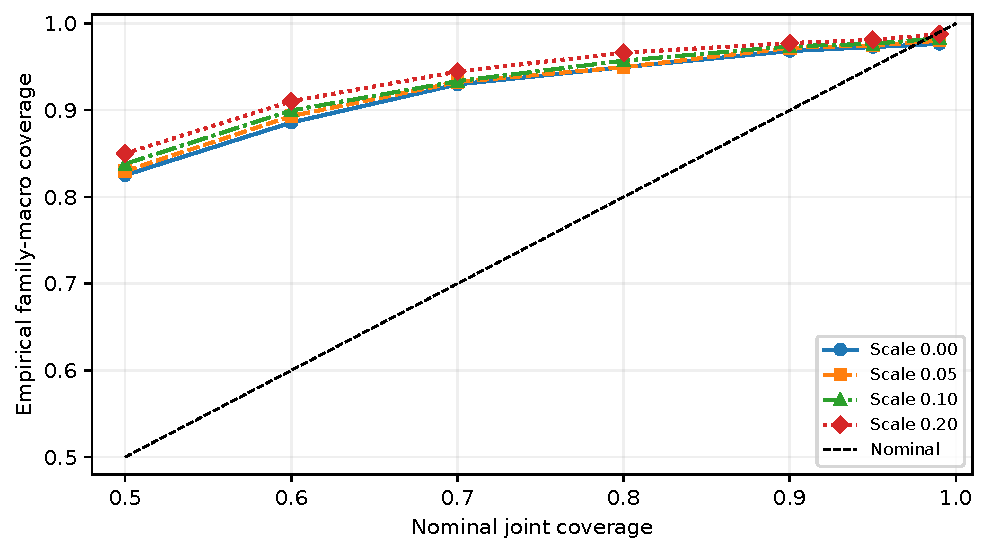
\includegraphics[width=.84\textwidth]{figures/support_coverage.pdf}
\caption{Post hoc empirical coverage at seven nominal levels, recalculated from saved predictions with the complete mean fixed. Symbols and line styles identify covariance scales. The diagonal indicates nominal coverage; no independent calibration sample or confidence bands are introduced.}
\label{fig:support_coverage}
\end{figure}

\subsection{Initialization Jacobian audit}
The input cache contains the physical derivative matrix $J$ and nuisance derivative matrix $J_n$ at the observation initializer. Residuals are divided by observation noise and physical perturbations are measured in prior-standard-deviation units. We reconstruct $J_\perp=J-J_nJ_n^+J$ using the recorded nuisance dimensions and a pseudoinverse cutoff of $10^{-8}$. It exactly matches the stored projected derivative in this cache. These are initialization derivatives, not final robust-anchor derivatives or separate setup-bounce derivatives. Singular values below $\max(10^{-10},10^{-8}s_{\max})$ count as zero.

\par\begin{table}[htbp]\centering\small
\caption{Post hoc singular-value audit of the active initialization subspace. Condition medians use full-rank rows. All entries are in the cache\textquotesingle s standardized coordinate system.}
\label{tab:support_jacobian}
\begin{tabular}{lrrrr}\toprule Protocol & Full rank / rows & Median $s_{\min}$ & 10th pct. $s_{\min}$ & Median condition\\\midrule
multiple forces & 360/360 & 0.6557 & 0.5532 & 11.3110 \\
unforced slide & 360/360 & 3.6974 & 3.4170 & 1.0000 \\
bounce & 360/360 & 21.0018 & 18.9655 & 1.0000 \\
\bottomrule\end{tabular}\end{table}\par

The one-dimensional condition number is identically one for a nonzero column and does not itself indicate strong information. Inactive derivative columns are zero by construction in the initializer; this audit therefore cannot establish that the protocol mask equals the null space of an unrestricted physical model. Initial full rank does not remove nonlinear contact ambiguity or guarantee stable posterior inference. In particular, full rank of the bounce initialization does not invalidate the empirically selected final fallback.


\Needspace{8\baselineskip}
\section{Independent frozen-video representation control}
This additional study was specified after the original results and is post hoc. It uses the official frozen V-JEPA 2 ViT-L encoder, repository \path{facebook/vjepa2-vitl-fpc64-256}, at the following pinned commit:
\par\noindent{\small\texttt{b3c1679b7c34d3255ef3547f27c7b226aefab26f}}\par
All 24,480 original frame files across 1,980 development and 1,080 previously evaluated episodes were hash-checked. Each clip contains exactly the original eight ordered RGB frames. No additional frames, temporal resampling, or physical target is used during feature extraction. Spatial preprocessing uses the encoder's 256-pixel center crop after its native resize, and encoder evaluation uses BF16. This differs from the Qwen path's spatial processing.

The final encoder tokens are averaged to 1,024 features. Centered PCA is fitted separately on each training fold and retains 48 components; the evaluation fold never fits the projection. The final projection uses all development features only. The existing numerical head, residual target, penalties, clipping, visual shrinkage, protocol masks, generalized-bounce fallback, and covariance rule are unchanged. The same six development family folds are used. This matches residual-stage rules and output dimension, but not encoder pretraining, observation-decoder supervision, or preprocessing. The PCA map additionally stores 49,152 loadings and 1,024 centering values; these are outside the original residual-coefficient count.

\begin{table}[htbp]\centering\small
\caption{Post hoc frozen-video control. Action errors are in millimeters. Development evaluates the residual stage using the original fixed upstream models. The final column gives the existing-cohort paired difference from the original full model and an unadjusted two-sided 95\% interval.}
\begin{tabular}{lrrl}\toprule
Configuration & Development & Evaluated & Difference from full [95\% interval]\\\midrule
Numerical only & 1.371928 & 1.468770 & $+0.01565\ [-0.00053,+0.03114]$\\
Original full & 1.352231 & 1.453122 & reference\\
V-JEPA 2, PCA-48 & 1.382427 & 1.470615 & $+0.01749\ [-0.00118,+0.03560]$\\\bottomrule
\end{tabular}\end{table}

The V-JEPA-minus-numerical difference is $+0.00185$ mm with interval $[-0.00914,+0.01288]$ mm on the existing evaluation cohort. The full model has the lower point error, but neither this comparison nor V-JEPA versus full establishes a two-sided directional difference. The development V-JEPA-minus-full difference is $+0.03020$ mm, with interval $[+0.01019,+0.05058]$ mm; it does not supersede the existing-cohort uncertainty. All planned configurations are reported without changing the primary model. V-JEPA's evaluated NLL/dimension, marginal CRPS, and joint 90\% coverage are $-2.543389$, $0.01318921$, and $0.973611$, respectively. Cached embeddings, the fixed plan, PCA maps, prediction arrays, and refitting code accompany the package.

\section{Upstream lineage and an RGB-path replay}
The saved observation-decoder training records identify 328,356 parameters, 720 training episodes, and 48 old-development geometry families. The training objective combines center-of-mass pixel supervision with fixed physical-response sensitivity terms. The frozen encoder is not trained in this stage. An identifier audit finds no episode or family-identifier overlap with the later 72-family confirmation cohort. This is an identifier-level check, not an independent proof of asset or perceptual disjointness. Training receipts and source contracts are supplied; upstream training itself was not rerun.

The residual-development cohort contains these 720 upstream training episodes. Consequently, its six-fold results concern residual fitting conditional on the previously trained decoder, not out-of-fold training of every learned component. This distinction also limits interpretation of the development comparison with a video encoder that lacks this task-specific decoder supervision. The original later geometry cohort remains the primary evaluation.

The common appearance prior is a separate upstream learned component. Its recorded plan uses 12,000 first-image mappings (2,538 unique image hashes), with 8,400 training and 1,200 validation rows including repeated appearances. A frozen full Qwen pass uses the prompt ``Describe only the visible appearance of the object.'' The final-token feature undergoes float32 layer normalization, followed by a linear six-output head for three transformed means and three softplus scales. The plan specifies seeds 17, 43, and 101, 100 epochs, and minimum validation Gaussian NLL checkpoint selection; the primary path uses the frozen seed-17 checkpoint. This shared prior is also present in the numerical residual control. These are recorded training specifications, not a fresh reproduction of prior training.

An additional prior-lineage audit checks actual image-file hashes. The 9,600 fitting/selection rows contain 2,036 unique first-image hashes. Against all 1,080 later confirmation episodes (5,703 unique frame hashes), episode identifiers, family identifiers, and byte-exact image hashes have zero overlap. The saved 100-epoch history also reproduces the reported seed-17 selection at epoch 6. This does not prove perceptual or underlying asset independence, or exclude foundation-model pretraining overlap. The identifier/hash tables, training plan, and selection receipts accompany the evidence archive.

The RGB reproduction archive selects the first eight cases of the original observation index without using outcomes, covering all three protocols. Starting from 64 original RGB frames, it regenerates the first-image prior, tracking, numerical observation initialization, Qwen vision and decoder features, robust physical solves, and locked residual predictions. Prior, tracking, initialization, pooled, and position-decoder arrays reproduce exactly in the recorded environment. The maximum transformed-mean discrepancy is $5.29\times10^{-10}$, and the maximum covariance-entry discrepancy is $6.06\times10^{-14}$. Before execution, absolute tolerances were set to $10^{-6}$ for prior outputs, $10^{-4}$ for numerical inputs and decoder features, and $10^{-5}$ for posterior entries. Reference arrays are used for assertions; physical targets do not enter prediction.

The archive includes required research modules and small checkpoints, while the pinned Qwen base weights are separately downloaded and hash-checked. An independently extracted copy passes the same assertions while a Python file-read guard rejects dependencies on the original research source/data checkout. It uses the existing Python 3.11/CUDA runtime, not a newly installed environment. To preserve the original prior-head CPU batch shape, eight features are zero-padded to 256 rows; the linear head has no cross-row operation. This checks eight inference paths, not upstream training or full-dataset reproducibility. Run \path{scripts/run_access_rgb_bundle.py} in the RGB archive with its explicit model directory. Run \path{tools/score_access_video_control.py} in the Overleaf archive with Python, NumPy, and SciPy to refit the frozen-video control from bundled embeddings; its outputs are written to \path{replayed/video_control/}.


\section{New-episode evaluation with disjoint friction conditions}
The follow-up plan was fixed after the original experiments but before downloading new videos or reading new displacement outcomes. It retains the pinned PhysProbe commit. The supplied metadata contain 16 distinct $(\mu_s,\mu_d)$ pairs for the object and 16 for the surface. These are physical material conditions, not identifiers for distinct cube assets or scenes. An audit finds that the original development/confirmation cohorts share 15 object-material and all 16 surface-material conditions.

All 192 formerly selected episodes and feasibility episodes 0--9 are excluded. Each material list is sorted, then ordered by SHA-256 of the fixed seed, axis name, and material tuple. Seed 2026091307 assigns the first eight materials per axis to training and the remaining eight to evaluation. Episodes must belong to the same role on both axes; the 630 mixed assignments are omitted. This produces 320 training and 348 evaluation candidates. The unchanged full-video visibility procedure retains 285 and 329, excluding 35 and 19 respectively. The package records exclusions by group. The evaluation contains 63 of 64 possible held-out material combinations. Video hashes have zero overlap across roles. Material values are used for grouping only and are not readout inputs.

The numeric-summary, temporal-visual, and quality-gate views are unchanged. Penalties remain 10, 1,000, and 0.1, respectively; there is no new hyperparameter search. Readout coefficients are newly fitted on the 285 training cases. For every observed training material pair, component models used to form gate targets exclude all rows with either of that pair's material conditions. The 58 such internal fits cover all training rows. The final numeric and visual components use all training rows, and the gate is fitted from these internally held-out predictions. Original checkpoints and paper results are retained. Architecture and penalty selection historically used other episodes from the same material bank; the separation applies to this refitting experiment, not to every preceding design decision.

Predictions for all 329 evaluation episodes were saved and hashed before any evaluation trajectory was downloaded. Only then were the planar displacement targets read. RGB processing uses the original eight frame offsets and 50 fps horizon; it retains offline full-video eligibility and is not a new causal-online protocol.

\subsection{Metric, crossed-material uncertainty, and result}
Let $\bar e^M_{ab}$ be method $M$'s mean vector error in millimeters among eligible episodes with object material $a$ and surface material $b$. For the 63 observed pairs $\mathcal C$, the primary difference is
\[
\Delta=|\mathcal C|^{-1}\sum_{(a,b)\in\mathcal C}
 (\bar e^{G}_{ab}-\bar e^{N}_{ab}).
\]
This gives each observed material pair equal weight. The secondary episode mean instead weights pairs in proportion to their episode counts. They estimate different averages and must not be interchanged when reporting the relative improvement.

For each of 20,000 bootstrap draws, eight object-material labels and eight surface-material labels are independently sampled with replacement. If their multiplicities are $w_a$ and $v_b$, a draw uses
\[
\Delta^*=\frac{\sum_{(a,b)\in\mathcal C}w_av_b
 (\bar e^{G}_{ab}-\bar e^{N}_{ab})}
 {\sum_{(a,b)\in\mathcal C}w_av_b}.
\]
The 2.5th and 97.5th percentiles form the reported interval. This applies the pigeonhole resampling principle to the observed material-pair means \cite{owen2007pigeonhole}. Missing cells are omitted; groups, not individual episodes, determine the crossed resampling weights. This is an approximate interval with only eight levels per axis, not an exact finite-sample guarantee, and it conditions on the fitted models and the visibility-selected data.

\begin{table}[htbp]\centering\small
\caption{Additional double-material holdout. The protocol was fixed before these new outcomes; it followed the earlier study. All errors are in millimeters.}
\begin{tabular}{lrr}\toprule Method & Equal material-pair MAE & Episode MAE\\\midrule
Numerical & 63.419394 & 65.091048\\
Raw visual residual & 61.942794 & 64.641735\\
Gated visual residual & 60.641429 & 62.753128\\\bottomrule
\end{tabular}\end{table}

The gated-minus-numerical difference is $-2.777965$ mm, or a 4.38\% material-pair reduction, with interval $[-6.043509,-0.115608]$ mm. Marginal mean differences, averaging observed pair means within each material, are negative in seven of eight object-material groups and five of eight surface-material groups. The fixed rule required a negative primary mean, a negative two-sided upper endpoint, and at least five improving groups on each axis; all three conditions pass. The upper endpoint is near zero. The result supports retention of the visual-plus-gate increment under held-out friction conditions in this refit, with the same cube/scene and previously selected architecture. It does not retroactively pass the original 10\% development rule, prove a separate gate-only effect, or establish new object/scene-asset generalization.

Run \path{tools/replay_group_holdout.py} to refit the models from supplied numeric/visual views, compare the sealed predictions, and replay the crossed-material interval. This uses NumPy and the included original readout routines. It does not re-extract all videos. The full observation plan, video hashes, eligibility records, feature provenance, training/evaluation targets, checkpoints, and predictions are under \path{evidence/group_holdout/}.


\section{Additional post hoc comparisons}\label{sec:extended}
All comparisons in this section were designed after the original outcomes were available. They are descriptive, outside the original analysis rules, with unadjusted intervals; the pooled 59-contrast Holm audit is provided in the follow-up section. The original models, primary bootstrap rule, and evaluated cohorts are unchanged. Hyperparameter selection uses development families only. The corresponding plan, raw numerical inputs, predictions, per-episode iteration records, and executable scripts are included in release v0.4.0.

\subsection{Iterated nonlinear anchors}
The additional fit minimizes $\frac12\|u\|^2+64\sum_t\rho(\nu_t)$, where $u$ is the active physical displacement from the original prior in prior-scale units and $\nu_t$ is the nonlinear observation residual divided by its original observation standard deviation. Each IRLS step recomputes Huber weights $\min(1,1.345/|\nu_t|)$ or Cauchy weights $[1+(\nu_t/2.385)^2]^{-1}$, and solves the weighted nonlinear least-squares problem with the original Gaussian physical prior. This differs from the primary anchor's frozen weights based on the initial unit-update innovation. Sliding retains free initial position/velocity with bounds $[-5,5]$ m and $[0,10]$ m/s; general bounce retains height/velocity/floor bounds $[-0.5,2]$, $[-2,2]$, and $[-0.4,0.5]$ in SI units. Setup bounce uses its original known height/velocity and free offset. Gravity is fixed.

We initialize at the original anchor and prior, use the same observation-derived nuisance initialization, and select the lower objective without targets. Inner SciPy trust-region least squares uses function/step tolerances $10^{-12}$, gradient tolerance $10^{-10}$, and at most 150 function evaluations. The outer loop stops when physical prior-unit and nuisance-coordinate changes both have norm below $10^{-8}$, or at 50 iterations. The nonlinear bounce solution remains local. Both robust methods converge for all 1,440 distinct episode/bounce-setup assumption fits (slide results are reused across bounce-setup assumptions); mean outer counts are 3.117 for Huber and 4.508 for Cauchy. Median changes from the original anchor are $1.28\times10^{-6}$ and $1.72\times10^{-5}$ in prior units, although a small movement in strongly informed coordinates can affect the trajectory metric.

The profiled Gaussian comparison minimizes $\frac12\|u\|^2+\frac{n}{2}\log[\max(\sum_t\nu_t^2/n,10^{-12})]$ by L-BFGS-B using the same starts, bounds, and prior. The likelihood scale is profiled per episode and no scale prior is added. The floor is a numerical safeguard, not a fitted hyperparameter. No floor activation occurs; 1,438 of 1,440 fits report optimizer convergence. The two remaining fits are retained and flagged, so its result is a bounded numerical comparison, not an all-cases convergence claim. Its mean iteration count is 26.156. Original residual heads are never transferred to or retrained on these new anchors.
\begin{table}[htbp]\centering\small
\caption{Post hoc anchor comparisons; full minus baseline with 20,000 paired family draws. Units are millimeters.}\label{tab:ext_anchor}
\begin{tabular}{lrrrr}\toprule
Baseline & MAE & Reduction (\%) & Difference & 95\% interval\\\midrule
Iterated Huber & 1.914820 & 24.112 & -0.461698 & $[-0.663424,-0.269751]$\\
Iterated Cauchy & 1.913327 & 24.053 & -0.460205 & $[-0.661572,-0.268427]$\\
Profiled MAP & 1.823148 & 20.296 & -0.370027 & $[-0.562096,-0.183656]$\\
\bottomrule\end{tabular}
\end{table}
\subsection{Protocol and coordinate breakdown}
Each table entry first averages episodes within a family and protocol, then families equally. The arithmetic mean of all six action cells reproduces each method's saved macro error within $10^{-12}$ meters. Sliding rows are identical across bounce-setup assumptions, not independent replications. The protocol decomposition against the original cell-specific best-of-robust/legacy reference differs from comparison against Huber alone: sliding accounts for 99.9\% of that reduction and unforced sliding for 61.8\%.
\begin{table}[htbp]\centering\small
\caption{Complete action decomposition (mm). G/S denote general/setup bounce-setup assumptions; M/U/B denote multiple-force, unforced, and bounce protocols.}\label{tab:ext_protocol}
\begin{tabular}{lrrrrrr}\toprule
Method & G-M & G-U & G-B & S-M & S-U & S-B\\\midrule
Unit & 3.633112 & 2.156062 & 0.791835 & 3.633112 & 2.156062 & 0.344740\\
Fixed Huber & 3.633112 & 2.156062 & 0.515000 & 3.633112 & 2.156062 & 0.352266\\
Fixed Cauchy & 3.638990 & 2.169002 & 0.516761 & 3.638990 & 2.169002 & 0.355631\\
Numerical & 3.020342 & 0.977727 & 0.515000 & 3.020342 & 0.977727 & 0.301482\\
Full & 2.989925 & 0.960083 & 0.515000 & 2.989925 & 0.960083 & 0.303715\\
Legacy & 3.901642 & 2.002216 & 0.792138 & 3.901642 & 2.002216 & 0.307627\\
RGB temporal & 4.249430 & 2.344330 & 0.782657 & 4.249430 & 2.344330 & 0.335869\\
Iterated Huber & 3.068313 & 2.086893 & 0.833767 & 3.068313 & 2.086893 & 0.344740\\
Iterated Cauchy & 3.068283 & 2.086901 & 0.824849 & 3.068283 & 2.086901 & 0.344743\\
Profiled MAP & 2.893515 & 2.071250 & 0.664873 & 2.893515 & 2.071250 & 0.344488\\
\bottomrule\end{tabular}
\end{table}
Coordinate errors below show family-macro mean / median of family mean absolute transformed-coordinate error. Inactive coordinates are N/A. Shared sliding rows are shown once; the downloadable CSV also contains their duplicate setup-bounce-setup assumption rows. This table measures estimation error, not nuisance error or an identifiability guarantee.
\begingroup\scriptsize
\begin{longtable}{llrrr}
\caption{Active-coordinate error by method and protocol.}\\
\toprule Method & Protocol & $\log m$ & $\log\mu$ & $\operatorname{logit}e$\\\midrule\endhead
Unit & Multiple & 0.04640 / 0.03933 & 0.05513 / 0.04507 & N/A\\
Unit & Unforced & N/A & 0.01371 / 0.01033 & N/A\\
Unit & General B & N/A & N/A & 0.01257 / 0.00359\\
Unit & Setup B & N/A & N/A & 0.00394 / 0.00300\\
Fixed Huber & Multiple & 0.04640 / 0.03933 & 0.05513 / 0.04507 & N/A\\
Fixed Huber & Unforced & N/A & 0.01371 / 0.01033 & N/A\\
Fixed Huber & General B & N/A & N/A & 0.00506 / 0.00301\\
Fixed Huber & Setup B & N/A & N/A & 0.00414 / 0.00302\\
Fixed Cauchy & Multiple & 0.04652 / 0.03953 & 0.05525 / 0.04565 & N/A\\
Fixed Cauchy & Unforced & N/A & 0.01380 / 0.01033 & N/A\\
Fixed Cauchy & General B & N/A & N/A & 0.00506 / 0.00307\\
Fixed Cauchy & Setup B & N/A & N/A & 0.00420 / 0.00307\\
Numerical & Multiple & 0.03147 / 0.02499 & 0.03182 / 0.02460 & N/A\\
Numerical & Unforced & N/A & 0.00633 / 0.00584 & N/A\\
Numerical & General B & N/A & N/A & 0.00506 / 0.00301\\
Numerical & Setup B & N/A & N/A & 0.00328 / 0.00267\\
Full & Multiple & 0.03111 / 0.02488 & 0.03177 / 0.02355 & N/A\\
Full & Unforced & N/A & 0.00619 / 0.00544 & N/A\\
Full & General B & N/A & N/A & 0.00506 / 0.00301\\
Full & Setup B & N/A & N/A & 0.00330 / 0.00266\\
Legacy & Multiple & 0.05082 / 0.04345 & 0.05874 / 0.05118 & N/A\\
Legacy & Unforced & N/A & 0.01239 / 0.01032 & N/A\\
Legacy & General B & N/A & N/A & 0.01266 / 0.00386\\
Legacy & Setup B & N/A & N/A & 0.00321 / 0.00276\\
RGB temporal & Multiple & 0.05361 / 0.04449 & 0.06527 / 0.05126 & N/A\\
RGB temporal & Unforced & N/A & 0.01461 / 0.01035 & N/A\\
RGB temporal & General B & N/A & N/A & 0.01248 / 0.00362\\
RGB temporal & Setup B & N/A & N/A & 0.00377 / 0.00312\\
Iterated Huber & Multiple & 0.03998 / 0.03512 & 0.04470 / 0.03547 & N/A\\
Iterated Huber & Unforced & N/A & 0.01321 / 0.00991 & N/A\\
Iterated Huber & General B & N/A & N/A & 0.01352 / 0.00361\\
Iterated Huber & Setup B & N/A & N/A & 0.00394 / 0.00300\\
Iterated Cauchy & Multiple & 0.03999 / 0.03514 & 0.04470 / 0.03548 & N/A\\
Iterated Cauchy & Unforced & N/A & 0.01321 / 0.00990 & N/A\\
Iterated Cauchy & General B & N/A & N/A & 0.01353 / 0.00353\\
Iterated Cauchy & Setup B & N/A & N/A & 0.00394 / 0.00300\\
Profiled MAP & Multiple & 0.03819 / 0.03086 & 0.04294 / 0.03579 & N/A\\
Profiled MAP & Unforced & N/A & 0.01309 / 0.01038 & N/A\\
Profiled MAP & General B & N/A & N/A & 0.00697 / 0.00321\\
Profiled MAP & Setup B & N/A & N/A & 0.00394 / 0.00300\\
\bottomrule\end{longtable}\endgroup
\subsection{Cross-fitted targets and shrinkage}
Five family-disjoint inner folds create numerical predictions for the visual targets inside each of six outer development folds. The final descriptive model uses five inner folds across all development families, then fits numerical and visual coefficients on all development data. Inner numerical normalization uses only its training families. Visual normalization uses the outer training data, as in the original model. Ridge penalties, masks, clipping, and shrinkage are fixed. The only changed learning target is the residual after an out-of-fold numerical prediction. No evaluated-family targets enter fitting or selection.
\begin{table}[htbp]\centering\small
\caption{Visual increment under the two target constructions. Intervals are paired differences from numerical-only, in mm.}\label{tab:ext_crossfit}
\begin{tabular}{lrrrr}\toprule
Cohort & Target & MAE & Increment (\%) & 95\% interval\\\midrule
Development & in sample & 1.352231 & 1.436 & $[-0.03773,-0.00131]$\\
Confirmation & in sample & 1.453122 & 1.065 & $[-0.03114,+0.00053]$\\
Development & crossfit & 1.350328 & 1.574 & $[-0.04228,-0.00046]$\\
Confirmation & crossfit & 1.451620 & 1.168 & $[-0.03446,+0.00095]$\\
\bottomrule\end{tabular}
\end{table}
The corresponding one-sided upper bounds on evaluated families are $-0.002189$ mm (original targets) and $-0.002213$ mm (cross-fitted targets). Both two-sided intervals include zero. The original full view improves 46/72 families; the exact two-sided binomial sign test is $p=0.02446$. That frequency null differs from the mean-difference bootstrap null, so the sign result is not substituted for the mean inference.

The shrinkage sweep changes only the fixed multiplier of the already clipped visual prediction; its training target and fitted coefficients are unchanged. Covariance is recomputed from the accepted total correction. The original 0.25 row reproduces the original full predictions and all scores to $10^{-12}$. The development point minimum at 0.50 does not trigger replacement of the original model.
\begin{table}[htbp]\centering\small
\caption{Post hoc visual-shrinkage sensitivity. Development is six-fold; evaluated results are descriptive.}\label{tab:ext_shrink}
\begin{tabular}{lrrrrr}\toprule
Cohort & Scale & MAE (mm) & NLL/dim. & CRPS & Coverage\\\midrule
Development & 0 & 1.371928 & -2.175173 & 0.013604 & 0.975000\\
Development & 0.1 & 1.362306 & -2.177212 & 0.013603 & 0.975000\\
Development & 0.25 & 1.352231 & -2.179550 & 0.013619 & 0.975505\\
Development & 0.5 & 1.347138 & -2.181497 & 0.013691 & 0.975000\\
Development & 1.0 & 1.385694 & -2.177991 & 0.014000 & 0.973485\\
Confirmation & 0 & 1.468770 & -2.542391 & 0.013136 & 0.973611\\
Confirmation & 0.1 & 1.460132 & -2.544056 & 0.013122 & 0.973611\\
Confirmation & 0.25 & 1.453122 & -2.545938 & 0.013113 & 0.973611\\
Confirmation & 0.5 & 1.447645 & -2.547442 & 0.013133 & 0.973611\\
Confirmation & 1.0 & 1.465189 & -2.544428 & 0.013299 & 0.974537\\
\bottomrule\end{tabular}
\end{table}
\subsection{Development-selected channels and direct regressors}
Combined, pooled-only, and position-only views each search penalties $\{1,10,100\}$ using six-fold development macro action error. The selected penalties are 10, 1, and 1. Dimension-specific columns are removed rather than padded; training means and standard deviations are recomputed within folds. Selection reuses development outcomes, so selected development scores are not unbiased generalization estimates. All evaluated-cohort comparisons remain descriptive. The full nine-point search is in \path{replayed/extended/channel_grid.csv}.

The deduplicated numerical view uses the nine varying channels at eight frames plus the 15 setup channels once, totaling 87. It searches $\{0.1,1,10\}$, selects 0.1, and retains the visual stage. This sensitivity does not replace the original 192-dimensional view. The original replication of constants effectively distributes regularization over repeated columns.
\begin{table}[htbp]\centering\small
\caption{Development-selected feature views; evaluated differences and intervals are relative to numerical-only. Units are mm.}\label{tab:ext_channels}
\begin{tabular}{lrrrr}\toprule
View & Penalty & Develop. & Evaluated & 95\% interval\\\midrule
full & 10 & 1.352231 & 1.453122 & $[-0.03114,+0.00053]$\\
pooled & 1 & 1.367114 & 1.467461 & $[-0.01873,+0.01721]$\\
position & 1 & 1.351154 & 1.451117 & $[-0.03101,-0.00512]$\\
deduplicated numeric & 0.1 & 1.347917 & 1.426315 & $[-0.07105,-0.01508]$\\
\bottomrule\end{tabular}
\end{table}
Direct ridge and MLP use the same 240 numerical-plus-visual input coordinates and predict all three transformed properties, without an anchor update or output mask. Known setup/prior information remains in the input features. Ridge penalties $\{0.1,1,10,100,1000\}$ are selected by five inner family folds inside each outer training set. The direct MLP has two 64-unit ReLU hidden layers and three outputs, AdamW with learning rate 0.001 and weight decay $10^{-4}$, and a 300-epoch cap. Training-family normalization is used for inputs and raw-coordinate targets; no anchor-standardized target is used. One of five inner family folds selects the epoch by standardized-coordinate MSE with patience 25, then all outer training families are refitted at that epoch. Seeds 17, 43, and 101 are averaged in prediction space. Final selected epochs are 60, 84, and 80. These are specified small-network baselines, not an exhaustive learned-system comparison, and no posterior is supplied.
\begin{table}[htbp]\centering\small
\caption{Post hoc direct-regression baselines. Difference intervals are relative to the original full model, in mm.}\label{tab:ext_direct}
\begin{tabular}{lrrr}\toprule
Method & Cohort & MAE & 95\% difference interval\\\midrule
RIDGE & Development & 32.399926 & $[28.51888,33.64795]$\\
RIDGE & Confirmation & 33.402860 & $[28.75547,35.34003]$\\
MLP & Development & 30.620605 & $[26.38529,32.34098]$\\
MLP & Confirmation & 26.489233 & $[22.42777,27.73870]$\\
\bottomrule\end{tabular}
\end{table}
\subsection{Engine-rollout proxy}
PyBullet DIRECT simulates a 0.01-m-radius sphere with zero rotational inertia, a plane with unit friction and restitution, zero damping, and estimated/true object coefficients. Gravity is 9.81 m/s$^2$, time step $1/480$ s, solver iterations 100, and restitution velocity threshold zero. The same force schedule, initial speeds, drop height, and eight evaluation times as the analytic metric are used. No image rendering or new observation extraction is needed: this is a downstream simulation of saved estimates. It is a nonrotating-contact proxy rather than a rerendering or dynamic validation of the original geometry assets. The plane/object coefficients combine through the engine's contact model. The saved engine trajectories and family losses allow independent metric replay without PyBullet; fresh rollouts require PyBullet (tested Linux build January 29, 2025, API 202010061).
\begin{table}[htbp]\centering\small
\caption{Controlled engine proxy and analytic metric, aggregated by family.}\label{tab:ext_engine}
\begin{tabular}{lrrrr}\toprule
Method & Engine MAE (mm) & Analytic MAE (mm) & Pearson & Spearman\\\midrule
Fixed Huber & 2.236155 & 2.074269 & 0.99251 & 0.98566\\
Numerical & 1.620483 & 1.468770 & 0.98035 & 0.96128\\
Full & 1.605715 & 1.453122 & 0.97954 & 0.96373\\
\bottomrule\end{tabular}
\end{table}
The full-minus-Huber paired interval is $[-0.83816,-0.44089]$ mm. Agreement of family rankings supports the analytic proxy within this controlled contact model, not independent real-world accuracy.
\begin{figure}[htbp]\centering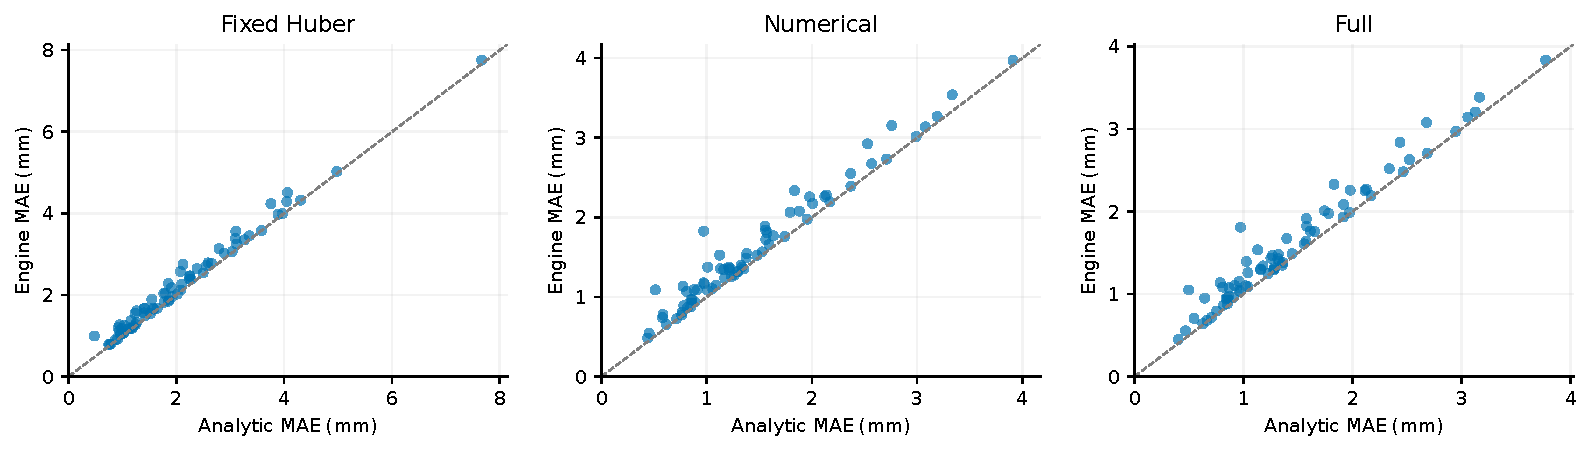
\includegraphics[width=.95\textwidth]{figures/engine_scatter.pdf}\caption{Post hoc family-level analytic and controlled-engine errors. Each panel has 72 families; no family is removed.}\end{figure}

\subsection{Public displacement scales}
Normalized MAE divides episode mean vector error by mean target-vector norm. Vector $R^2=1-\sum_i\|\hat y_i-y_i\|^2/\sum_i\|y_i-\bar y\|^2$. These are episode-weighted descriptors, separate from the primary equal-material-pair MAE. A mean predictor fitted on development may have slightly negative evaluation $R^2$; a predictor set to the evaluation mean is an oracle sanity check with exactly zero $R^2$, not a baseline selected on evaluation targets.
\begin{table}[htbp]\centering\small
\caption{Target displacement-norm distribution (mm).}\label{tab:ext_scale}
\begin{tabular}{lrrrrrr}\toprule
Split & n & Mean & Median & SD & Q25 & Q75\\\midrule
Episode & 123 & 193.869 & 215.989 & 64.589 & 179.374 & 229.273\\
Material & 329 & 190.281 & 213.097 & 57.974 & 170.110 & 226.632\\
\bottomrule\end{tabular}
\end{table}
\begin{table}[htbp]\centering\small
\caption{Episode-normalized public errors and vector coefficients of determination.}\label{tab:ext_r2}
\begin{tabular}{lrrr}\toprule
Split & Method & Normalized MAE & $R^2$\\\midrule
Episode & constant prior & 0.681551 & -0.004428\\
Episode & numeric & 0.382638 & 0.621118\\
Episode & raw vlm & 0.367309 & 0.661853\\
Episode & gated vlm & 0.366303 & 0.658853\\
Material & numeric & 0.342079 & 0.634251\\
Material & raw & 0.339718 & 0.649059\\
Material & gated & 0.329793 & 0.657154\\
\bottomrule\end{tabular}
\end{table}
\subsection{Recorded inference-time components}
One hundred outcome-free selected episodes (34 multiple-force, 33 unforced, 33 bounce) are measured at batch size one, with CUDA synchronization around GPU stages. Model loading is excluded; totals sum components measured in separate model-resident passes. They are not contiguous cold-start or deployment throughput benchmarks. The shared first-image prior remains in both paths; a fully VLM-free baseline would be a different model. Tracking/initialization includes its required image work, and visual preprocessing includes its own image loading. Hardware: NVIDIA GeForce RTX 5080, driver 591.86, CUDA 12.8, PyTorch 2.11.0+cu128, Python 3.11.9, Windows build 26200. The setup-bounce row uses only its 33 applicable episodes and is already included in the robust-fit total, not added twice.
\begin{table}[htbp]\centering\small
\caption{Measured latency components (milliseconds); 100 episodes except the setup-bounce subset.}\label{tab:ext_latency}
\begin{tabular}{lrrr}\toprule
Stage & Median & Q25 & Q75\\\midrule
First-image prior & 68.394 & 60.705 & 81.938\\
Additional frame preprocessing & 15.747 & 15.373 & 16.096\\
Eight-frame vision encoder & 179.167 & 177.558 & 181.665\\
Observation decoder & 32.741 & 31.952 & 40.214\\
Tracking / initialization & 37.570 & 36.221 & 51.689\\
Robust fits, both bounce-setup assumptions & 17.523 & 16.159 & 43.753\\
Setup bounce, 75 calls (subset) & 16.869 & 16.643 & 17.350\\
Residual heads & 0.342 & 0.319 & 0.353\\
Shared-prior / anchor component sum & 129.067 & 117.546 & 163.849\\
Full component sum & 362.528 & 345.832 & 396.436\\
\bottomrule\end{tabular}
\end{table}
The exact measurement source and all 100 timing rows are retained. Portable replay verifies those recorded quantiles; it does not recreate timings on a different computer. New measurement requires the source's original RGB inputs and upstream model environment. General bounce uses 81 forward evaluations in the original kernel, whereas setup bounce uses 75; these distinct budgets are not conflated.

\subsection{Bounce and real-video diagnostics}
The bounce diagnostics compare the unclamped branch's learned standardized correction with its true standardized target, without changing the deployed fallback. Fold-wise correlations, clipping rates, scales, and target dispersion are provided in \path{replayed/extended/bounce_diagnostics.csv}. The evaluated rows are shown below. Training numerical clipping rate is zero for the full development fit; visual prediction clipping occurs only in general bounce. Similar median anchor scales alongside very different residual-target dispersion favor a predictability explanation over an unsupported claim of uniformly inflated covariance. The role of free nuisance coordinates is not causally isolated.
\begin{table}[htbp]\centering\small
\caption{Evaluated bounce residual diagnostics; each bounce-setup assumption has 360 episodes.}\label{tab:ext_bounce}
\begin{tabular}{lrrrr}\toprule
Bounce setup & Correlation & Visual clip rate & Median scale & Target SD\\\midrule
Generalized & 0.185769 & 0.063889 & 0.007517 & 2.264421\\
Setup & 0.501755 & 0.000000 & 0.007098 & 0.571314\\
\bottomrule\end{tabular}
\end{table}
The original real-video diagnostic is a scalar feature score, not a physical-property prediction, and does not invoke the appearance prior. Its mean (0.05614) and SD (0.04048) differ from the synthetic unforced visual score (0.00619 and 0.02482), but their motion-feature units are not matched: real inputs use projected pixels and synthetic inputs use shifts divided by tracking noise. This contract difference is directly visible in the supplied extraction sources. Therefore a calibrated property-distribution comparison and attribution of failure to the appearance prior are not applicable to this diagnostic.

The combined, pooled-only, and position-only real-score family correlations are $-0.700$, 0.027, and $-0.455$. The recorded 95\% family-bootstrap interval for the combined score is $[-0.972,-0.108]$. Tracking uses MIL with an overlay-derived initial cue, not red-component segmentation. The recorded tracker failure count is zero on 33 videos; its effectively fixed-size boxes cannot validate object-size accuracy. Saved centroid second-difference roughness has Spearman 0.558 with family absolute rank error, but this is an unlabeled smoothness proxy, not a ground-truth tracking-error measurement or a causal explanation. The follow-up section corrects the noise-normalization contract and reruns these scores; the negative combined ranking persists. Independent tracking labels and a new evaluation cohort are still required for causal attribution.


\section{Strong-Anchor and Representation Follow-Up}
The follow-up specification is a timestamped local plan, not public preregistration. All added comparisons on previously evaluated families are exploratory. The original evidence files are hash checked and the original numerical/full predictions are re-fitted to absolute tolerance $10^{-12}$ before each numerical analysis. Focal comparisons do not replace the historical locally locked decision rules.

\subsection{Anchor ladder and a VLM-free estimator}
The Laplace control fits the joint physical/nuisance Gaussian MAP under original bounds and observation precision. A Gauss--Newton local Gaussian approximation is marginalized over nuisance by a Schur complement. Its physical mean equals the joint mode; it does not integrate a non-Gaussian posterior or profile dispersion. All 1,440 distinct fits converge, with no nuisance-bound contact or rank deficiency. The VLM-free profiled-MAP control uses a development population prior and observation-derived nuisance starts, with no appearance features or original-prior initialization. It uses the same cached calibrated RGB tracking measurements, and is not a matched residual-head ablation. One failed fit is retained.

\begin{table}[htbp]\centering\small
\caption{Added Classical Controls}\label{tab:fu_anchors}
\begin{tabular}{lrr}\toprule
Method & MAE (mm) & Convergence\\\midrule
Laplace marginal & 1.918031 & 100.00\%\\
VLM-free population MAP & 1.866472 & 99.93\%\\
\bottomrule\end{tabular}
\end{table}
\subsection{Matched dimensionality and missing numerical cell}
The 87-dimensional view concatenates nine dynamic channels across eight frames (72 values) with one copy of 15 setup channels. Numerical penalties $\{0.1,1,10\}$ use the original six family folds; 0.1 minimizes the numerical-only development loss. The four visual representations are compared above that same numerical fit. Their penalties $\{1,10,100\}$ use the same folds; neither evaluation targets nor errors select any setting. Development scores remain selection scores. The PCA fitting sets exclude validation families, and all final fits use development families only.

\begin{table}[htbp]\centering\small
\caption{Representation Ladder with Development-Selected Penalties}\label{tab:fu_repr}
\begin{tabular}{lrrrr}\toprule
Arm & Numeric $\lambda$ & Visual $\lambda$ & Dev. mm & Eval. mm\\\midrule
numeric192 & 1 & 0 & 1.37193 & 1.46877\\
full192 & 1 & 10 & 1.35223 & 1.45312\\
numeric87 & 0.1 & 0 & 1.36567 & 1.44213\\
qwen87 & 0.1 & 10.0 & 1.34792 & 1.42632\\
flow87 & 0.1 & 1.0 & 1.35202 & 1.41695\\
pixels87 & 0.1 & 100.0 & 1.36595 & 1.43405\\
vjepa87 & 0.1 & 100.0 & 1.37007 & 1.44407\\
\bottomrule\end{tabular}
\end{table}
The classical extractor uses only the same eight hash-checked grayscale RGB frames and the original first-frame object cue. Up to 64 ROI corners are propagated with pyramidal Lucas--Kanade (21-pixel window, three pyramid levels, 30 iterations, 0.01 tolerance). Median point displacement defines a centroid trajectory. The 48 features are seven horizontal and seven vertical displacements, six horizontal and six vertical second differences, seven horizontal direction cosines, seven point-spread ratios, and eight aggregate flow/failure/appearance-change statistics. Image dimensions normalize displacement. Zero successful tracks yields zero displacement and a failure count; no episode is removed. The evaluation set has 1,189 failed transitions of 7,560. Raw pixels are eight 16-by-16 grayscale frames followed by training-fold PCA-48. These controls are specified implementations, not optimized non-neural performance bounds. DINO, ResNet and text-generation arms are not claimed as completed. Upstream decoder supervision is not matched across encoder families.

\begin{figure}[htbp]\centering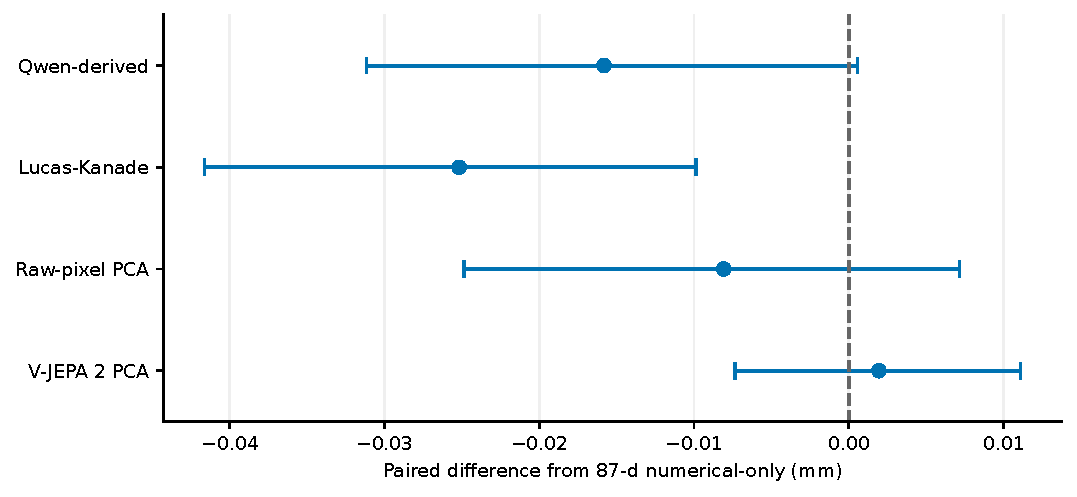
\includegraphics[width=.9\textwidth]{figures/representation_ladder.pdf}
\caption{Exploratory paired 95\% mean-error intervals relative to the strengthened numerical comparator. Interval overlap or inclusion of zero is not evidence of equivalence.}\end{figure}
\subsection{Multiplicity and effect interpretation}
Three focal comparisons use 20,000 paired family draws and two-sided sign-flip mean tests, with Holm adjustment within those three. A broader sensitivity applies Holm to 59 unique available family-action comparisons, removing duplicate prediction vectors and retaining unsuccessful baselines. The full list is in \path{replayed/followup/global_action_holm.csv}. This correction does not undo adaptive study history, selected penalties or repeated cohort use. Public episode bootstrap contrasts, correlation diagnostics, and covariance summary curves concern different estimands and remain explicitly descriptive; they are not new confirmatory discoveries. No statistical equivalence margin was specified.

\begin{table}[htbp]\centering\small
\caption{Focal Exploratory Contrasts (72 Families)}\label{tab:fu_focal}
\begin{tabular}{lrrr}\toprule
Contrast & $\Delta$ mm & 95\% interval & Holm $p$\\\midrule
full192 minus profiled MAP & -0.37003 & [-0.56199, -0.18024] & 0.00150\\
qwen87 minus flow87 & +0.00936 & [-0.01054, +0.03061] & 0.37728\\
qwen87 minus numeric87 & -0.01582 & [-0.03114, +0.00057] & 0.10139\\
\bottomrule\end{tabular}
\end{table}
\subsection{Capacity and latency}
Stored coefficient counts include intercepts and both setup branches: 1,544 numerical plus 392 visual coefficients for the original full model, and 704 plus 392 for the deduplicated full model. Excluding the generalized-bounce fallback branch yields 959 active coefficients for the deduplicated full model. The 328,356-parameter upstream observation decoder is separately trained and is excluded from these residual counts. PCA storage and encoder weights are not residual coefficients. The original component sums (129.1 and 362.5 ms) use staged model-resident GPU measurements; the 68.4-ms first-image prior is shared. Classical feature extraction is measured separately and cannot be added to those GPU totals to claim end-to-end acceleration. No full-path timing is imputed for unmeasured arms.
\begin{figure}[htbp]\centering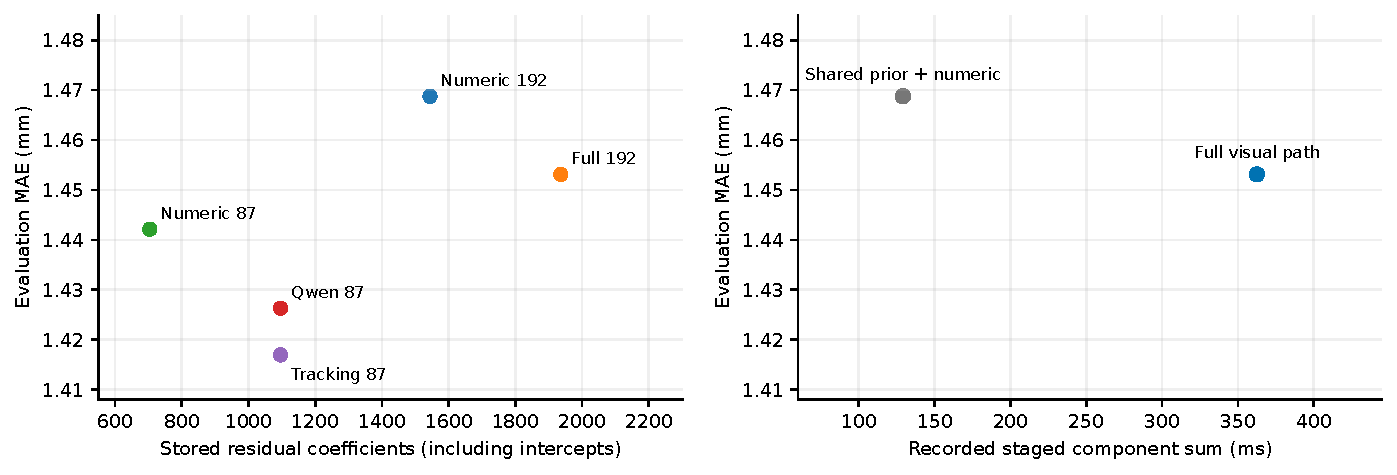
\includegraphics[width=\textwidth]{figures/capacity_latency.pdf}
\caption{Residual capacity versus error, and the two existing full-path component measurements. Neither panel isolates pretraining; the right panel omits unmeasured timings.}\end{figure}
\subsection{Feature-unit correction in real video}
The original 33-video inference is reconstructed with exactly matching raw scores. Both projected pixel-correction channels are divided by a tracking-noise proxy: 1.4826 times quadratic-detrended median absolute deviation, floored at one resized-image pixel. The resulting scale spans 1.000--1.077 pixels, so the intervention is small. Pooled states are unchanged. The operation matches dimensional form, not camera geometry or domain distributions. The 152-frame bridge uses deceleration/initial-speed and a camera indicator; scaling both numerator and denominator leaves the ratio invariant. Its scalar proxy is invariant for the same reason. The corrected short score is still not a friction estimate.

\begin{table}[htbp]\centering\small
\caption{Original and Unit-Normalized Real-Video Correlations}\label{tab:fu_real}
\begin{tabular}{lrrr}\toprule
Arm & Stage & Family $\rho$ & Bootstrap 95\%\\\midrule
combined & original & -0.700 & [-0.972, -0.121]\\
combined & noise\_normalized & -0.700 & [-0.972, -0.121]\\
pooled & original & 0.027 & [-0.571, 0.735]\\
pooled & noise\_normalized & 0.027 & [-0.571, 0.735]\\
position & original & -0.455 & [-0.944, 0.306]\\
position & noise\_normalized & -0.455 & [-0.944, 0.306]\\
kinematic\_short & original & 0.127 & [-0.713, 0.793]\\
kinematic\_short & noise\_normalized & 0.127 & [-0.713, 0.793]\\
bridge\_152frame & original & 0.355 & [-0.411, 0.869]\\
bridge\_152frame & normalized & 0.355 & [-0.411, 0.869]\\
scalar\_152frame & original & 0.427 & [-0.310, 0.906]\\
scalar\_152frame & normalized & 0.427 & [-0.310, 0.906]\\
\bottomrule\end{tabular}
\end{table}
\subsection{Independent-family calibration}
Forty new geometry families (600 RGB episodes) are generated using separate geometry and physics seed streams. Physical shape hashes are checked against prior geometry manifests. Generation-side targets are stored separately. The predictor is denied access to the target directory and records a hash/timestamp seal before calibration labels are opened. The original appearance prior, observation decoder and residual checkpoint are frozen. No model is fitted to calibration labels. Beta is selected by development CRPS, with no evaluation-coverage tuning.

For each family a fixed seed chooses one of its 30 episode/setup combinations uniformly, independently of residual values. The 37th order statistic of 40 normalized Mahalanobis scores defines the representative-family conformal scale. Its exchangeability target is a randomly sampled episode/setup of a new family. A separate 37th order statistic of within-family maxima targets simultaneous coverage of all such observations. Marginal and simultaneous-family coverage are different events; neither implies protocol-conditional nominal coverage. Evaluation on the previously inspected 72 families is descriptive and was not used to choose the quantile.
The selected $\beta$ is 0; representative-family $\hat q=0.44212$ and maximum-family $\hat q=7.91249$.

\begin{table}[htbp]\centering\small
\caption{Independent-Calibration Coverage on the Existing Evaluation Set}\label{tab:fu_cal}
\begin{tabular}{lrrr}\toprule
Region & Protocol & Coverage & Family-all\\\midrule
Unscaled & all & 96.81\% & 68.06\%\\
Unscaled & multiple forces & 91.94\% & 73.61\%\\
Unscaled & unforced slide & 100.00\% & 100.00\%\\
Unscaled & bounce & 98.47\% & 90.28\%\\
Representative & all & 81.94\% & 13.89\%\\
Representative & multiple forces & 67.22\% & 34.72\%\\
Representative & unforced slide & 91.94\% & 77.78\%\\
Representative & bounce & 86.67\% & 40.28\%\\
Family maximum & all & 99.86\% & 95.83\%\\
Family maximum & multiple forces & 100.00\% & 100.00\%\\
Family maximum & unforced slide & 100.00\% & 100.00\%\\
Family maximum & bounce & 99.58\% & 95.83\%\\
\bottomrule\end{tabular}
\end{table}
The public 53-episode empirical calibration is preserved and is not promoted to split conformal. A new independent public material-calibration partition is not implemented here. The new synthetic calibration assesses only its stated family sampling regime and fails the specified episode-coverage target; evaluation outcomes are not used to retune it.
\subsection{Scope of implemented extensions}
The protocol mask remains an assumption-driven restriction supported by elementary dynamics, not a newly proved Fisher-information rule. A final-solution automatic-mask policy, matched-supervision encoder 2-by-2 experiment, external text/simulator method ports, and three-axis asset/physics/sensor stress study are not included. The new independent geometries are calibration samples, not a model-misspecification or multi-object transfer benchmark. No equivalence or language-pretraining conclusion relies on missing cells. The original direct-regression and failed-transfer results remain in the preceding exploratory sections.


\section{Scope of available evidence}
The archives identify computational artifacts rather than distinct independent replications. The original public development result remains below its 10\% criterion. The controls do not isolate language pretraining, validate a general coordinate mask, or establish universal safety or coverage guarantees. The original cohorts have no independent calibration partition; the subsequent 40-family synthetic calibration is reported separately. Measured latency component sums are distinguished from contiguous end-to-end latency. The new material holdout retains the historical architecture-selection and shared-asset limitations described above.

\begingroup\small
\section{Portable calculation reproduction}
The companion source project compiles with pdfLaTeX and BibTeX. The main document is \path{main.tex}. Select \path{supplementary.tex} for this supplement or \path{cover_letter.tex} for the cover letter.

For numerical replay, install NumPy and run these commands outside Overleaf. Outputs are written to \texttt{replayed/}.
\begin{verbatim}
python tools/replay_tables.py
python tools/effect_sensitivity.py
python tools/run_support_study.py
python tools/score_access_video_control.py
python tools/replay_prior_lineage.py
python tools/replay_group_holdout.py
python tools/run_extended_study.py
python tools/run_followup_study.py
\end{verbatim}
The support and video studies additionally require SciPy. The extended runner refits robust baselines, cross-fitted targets, shrinkage/channel/direct controls, then replays public scales, real-score and latency diagnostics. Direct MLP fitting requires PyTorch; fresh engine execution requires PyBullet and is invoked separately with \texttt{python tools/engine\_rollout\_metric.py}. Individual script names and requirements are listed in \path{tools/README_extended.md}. Their feature caches and numerical kernels enable CPU refitting and scoring. Input hashes and the analysis plans are supplied under \path{evidence/support/} and \path{evidence/video_control/}. The prior-lineage command checks the supplied identifier/hash tables and selection receipts; it does not rehash the complete original image collection.

The separate \path{IEEE_Access_RGB_Reproduction.zip} includes a README, recorded environment versions, a pinned base-model download helper, and the eight-case offline runner. Its directory structure is independent of this Overleaf project. After obtaining the base model, run:
\begin{verbatim}
python scripts/run_access_rgb_bundle.py --model-dir /path/to/qwen
\end{verbatim}
The checks and discrepancies are written under \path{reproduced/}. Foundation weights are separate inputs. This example regenerates the first-image prior and executes the physical solver; it does not train upstream components or validate a fresh environment installation.

\begin{thebibliography}{S1}
\bibitem[S1]{owen2007pigeonhole} A. B. Owen, ``The pigeonhole bootstrap,'' \emph{The Annals of Applied Statistics}, vol. 1, no. 2, pp. 386--411, 2007, doi: \href{https://doi.org/10.1214/07-AOAS122}{10.1214/07-AOAS122}.
\end{thebibliography}
\endgroup
\end{document}
